\chapter{Related Work}

\label{ch:relatedwork}

\section{Workload-Aware Frameworks}

\subsection{Database Cracking}

From Idreos et al., Cracking is a relational database auto-tuning technique which performs online
restructuring of a relational table into disjoint pieces, storing information about each piece within
a separate data-structure called the cracker index.

When a column is queried, it is copied into a version of the column called the cracker column. The
cracker column is then scanned, restructuring it in-place to position the retrieved elements in
contigious positions. The indices of the bounds of the newly formed contigious region are stored
within the cracker index to inform future queries of whether they need to scan that piece of the
column.

Figure \ref{fig:cracking_img} shows two queries being run against a column within a system employing
database cracking. We can see that Q1 partitions copies the column into a cracker column, which is
then partitioned into pieces, of which information is known about the contents. Q2 further breaks
up the column into pieces, and again the information about the newly formed partitions is stored
in the cracker index.

\begin{figure}[h]
  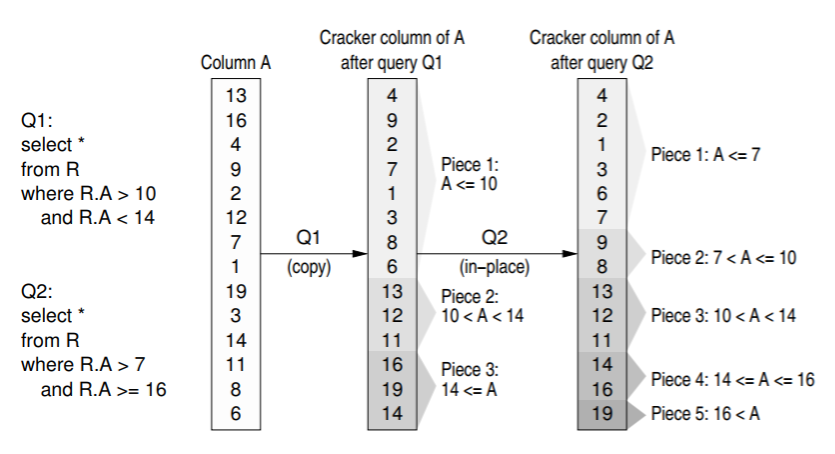
\includegraphics[width=\textwidth]{cracking_img}
  \caption{Illustration of database cracking}
  \label{fig:cracking_img}
\end{figure}

\subsection{Group-by-Query}

In-part inspired by cracking was the thesis work of Aluç, who proposed a group-by-query (G-by-Q)
representation for RDF data, for which the structure of individual database records, as well as
the way records are serialized on the storage system are dynamically determined based on the
workload. This technique proved to be fast and robust against other popular frameworks for
querying RDF data, however, the system is complicated - Aluç's implementation was reported to be
over 35,000 lines of C++. In this work we are aiming to produce simpler contributions.

\section{Graph Processing Frameworks}

\subsection{Ligra Framework}

Ligra is a lightweight graph processing framework for shared-memory multi-core machines for graph
traversal algorithms, such as pagerank and BFS. They were in part inspired by Beamer et al.'s work
with shared-memory machines, acheiving speed-up by dynamically switching between push and pull implementations of BFS based on the graph's density. Ligra takes the form of a simple API of three
routines: size, edgeMap and vertexMap.

size takes a set of vertices and returns the number of them.

edgeMap applies a function F to all out-neighbours of a vertex U which satisfy the condition C.

vertexMap applies a function F to every element in a set of vertices.

\section{Graph Indices}

\subsection{Space filling curve layouts}

The most famous example of this is the Hilbert Curve, which is a continuous mapping between a number
and a point on a 2D square. Numbers which are closeby are mapped closely together - in this way the
hilbert ordering of an index of an adjacency list is somewhat locality preserving. We can use a
hilbert ordering in order to improve locality on edge accesses, which therefore leads to improved
cache performance.

Another example of using a space filling curve to preprocess graph data is with co-ordinate 

\subsection{Frequency Based Clustering}

Frequency based clustering constitutes physically reorganising the vertex data such that frequently
accessed vertices are clustered. This improves cache utilisation and reduces the cycles spent stalled
on memory.
